% !TEX root = ../main.tex
\subsubsection{Geometry Effect}
\label{14.12::geometry_effect}
    % The effect has already been presented and discussed before, so we're brief.
    This problem has already been extensively discussed in Section \ref{12.42::geometry_effect}.
    In summary, the FMT detector is located at approximately $z \approx 26$ cm, and it exhibits poor performance for targets located too close to it.
    The strength of this effect can be quantified by applying the geometry cut described by Equation \eqref{eq::12.42::fmt_geometry_cut} to both the DC and FMT tracks.
    Figure \ref{fig::14.12::vz_012016_geomcut} illustrates the impact of this cut on both the DC and FMT tracks when applied to Figure \ref{fig::14.11::vz_seasons}.
    The effect of the cut on a $v_z$ vs $\theta$ plot can be observed in Figure \ref{eq::12.42::vz_vs_theta}.

    Based on this cut and the FMT's position along the $z$-axis, subsequent plots will be confined to the range $-30 \text{cm} < v_z < 20 \text{cm}$.
    In addition, unless otherwise specified, the cut is applied for all subsequent plots.

    \begin{figure}[h!]
        \frame{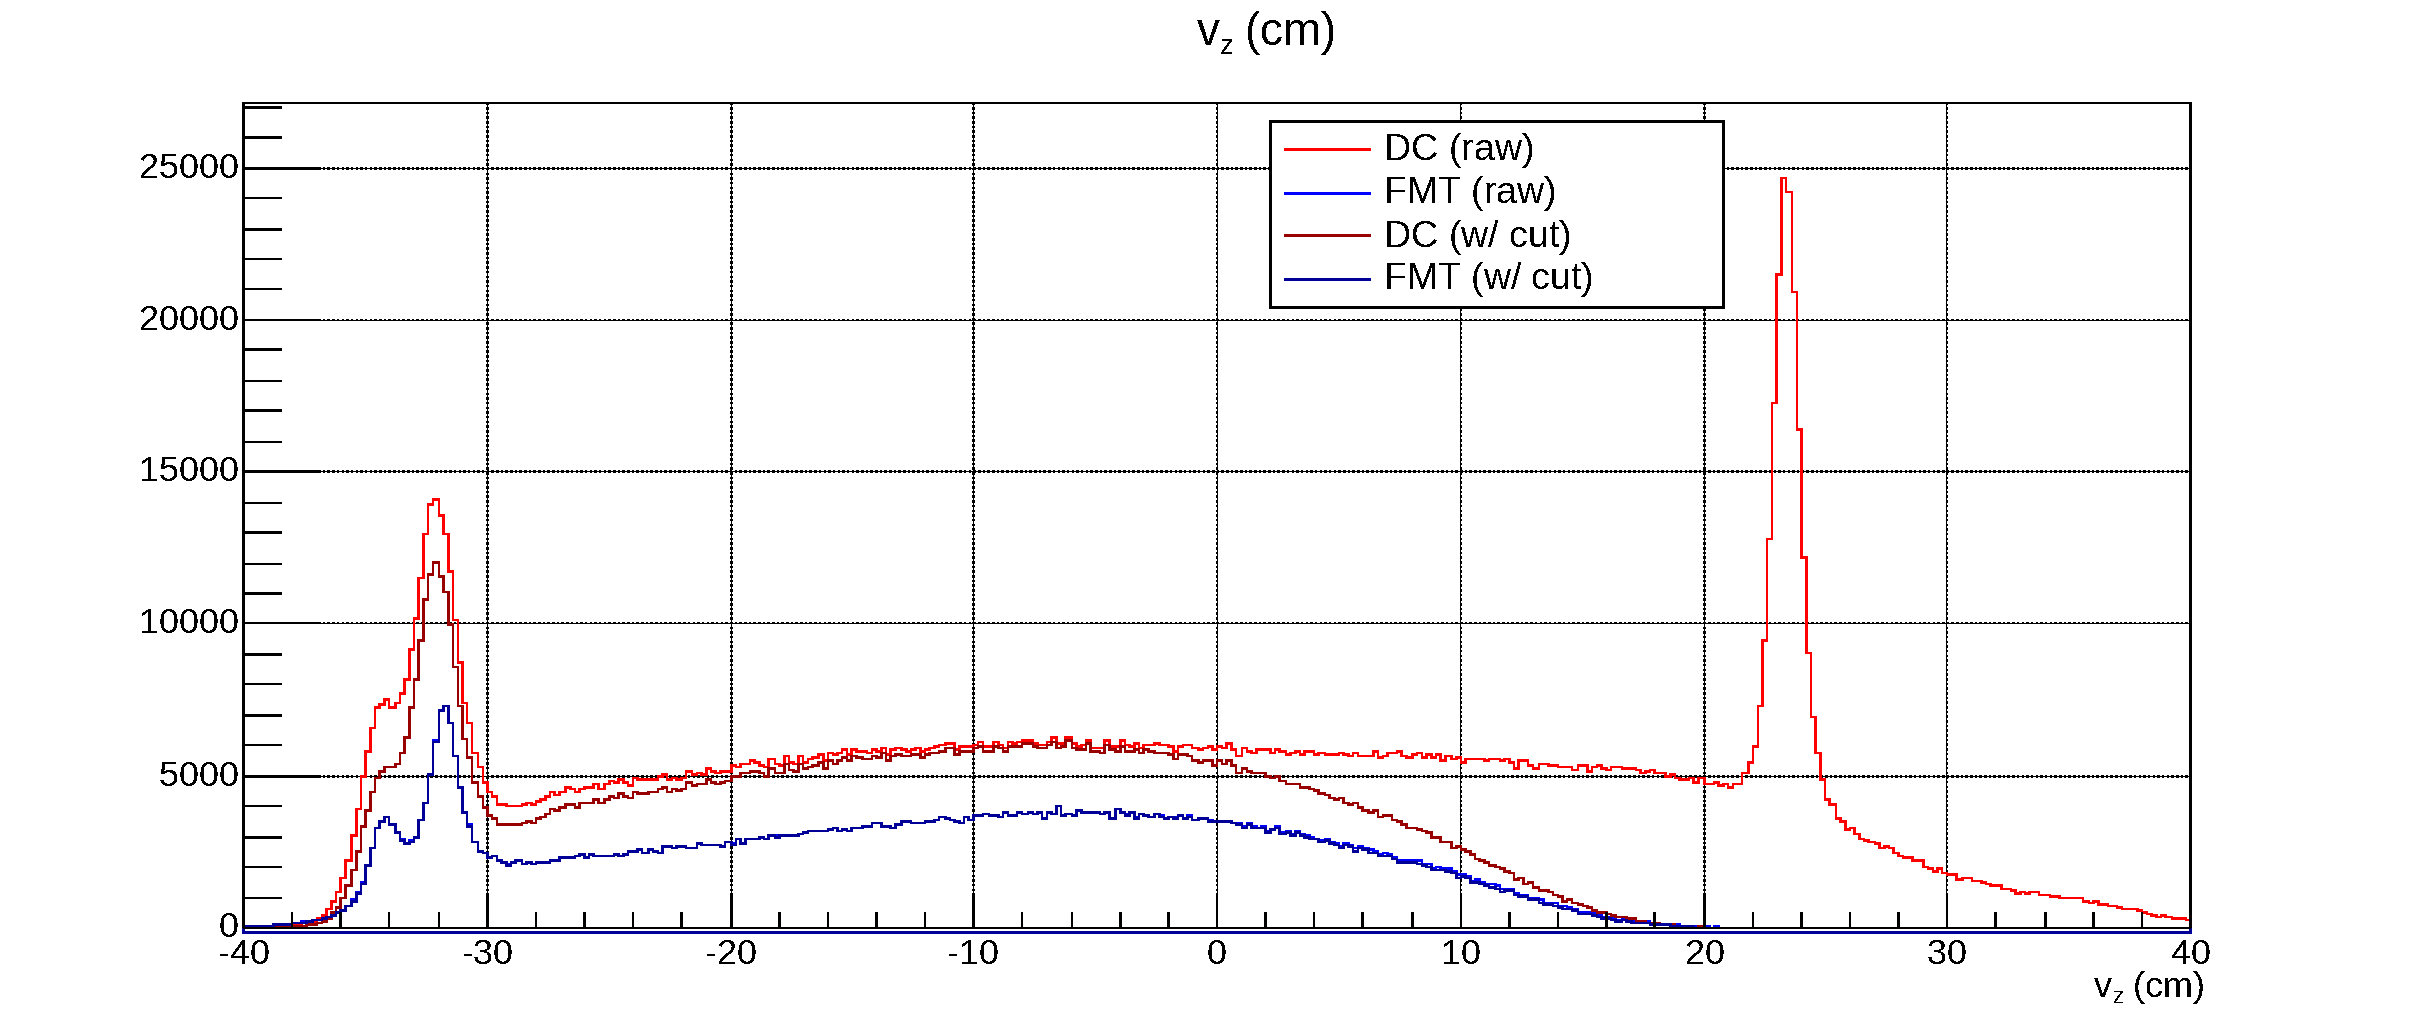
\includegraphics[width=\textwidth]{12vz_012016_geomcut.pdf}}
        \caption[$v_z$ for DC and FMT, w/ and w/out the geometry cut, run 12016]
        {$v_z$ for DC without the geometry cut (in red), with it (in dark red), for FMT without it (in blue), and with it (in dark blue).
        Spring 2020 data, run 12016.
        The effect of the cut is very clear on DC tracks, yet it almost doesn't affect FMT tracks.}
        \floatfoot{Source: Own elaboration, using the \href{https://github.com/bleaktwig/clas12-rge-analysis}{clas12-rge-analysis} software.}
        \label{fig::14.12::vz_012016_geomcut}
    \end{figure}
